
\chapter{Scenarios}


''Zacząłbym jakoś tak:
\\
To allow a researcher to evaluate learning agents in conditions of different characteristics, we provide a mechanism of scenarios.
\\
In this chapter we describe…''

To apply reinforcement learning we need a reward-driven environment. Modern state-of-the art AI solutions are not mature enough to cope with fully-fledged FPS game so availability of scenarios with simpler tasks and more transparent task-reward mechanics is crucial.\\
\\
Creation of scenarios is nice and easy so we created a couple of sample scenarios to show how it all works.\\
\\
\section{Definition}
What a scenario is, what it does and what it does not.

\section{Tools}
A few words about Doom Builder 2, acs scripts, reference to zdoom wiki, screen from doom builder 2.

\section{Advices?}
How to easily achieve some most common tasks in acs scripts which are not so obvious and were used here.
e.g. shaping rewards, infinite ammo, respawning, friendly monsters, 


\newpage
\section{Scenarios}
\subsection{Basic}
	\begin{figure}[h]
		\centering
		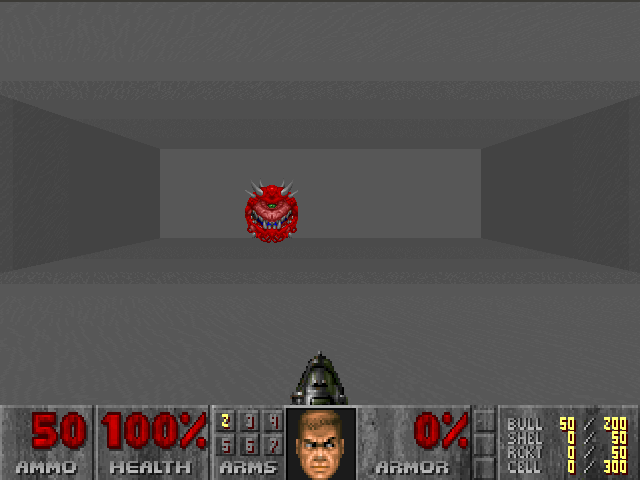
\includegraphics[scale=0.5]{basic.png}
		\caption{Doom gameplay frame from ''basic'' scenario}
	\end{figure}
\begin{itemize}
	\item motivation
	\item description
\end{itemize}

\newpage
\subsection{Deadly Corridor}
	\begin{figure}[h]
		\centering
		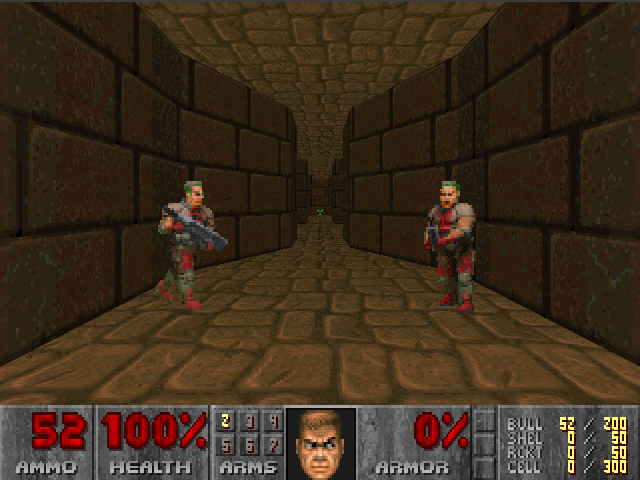
\includegraphics[scale=0.5]{deadly_corridor.png}
		\caption{Doom gameplay frame from ''deadly corridor'' scenario}
	\end{figure}
\begin{itemize}
	\item motivation
	\item description
\end{itemize}
\newpage

\subsection{Defend the Center}
	\begin{figure}[h]
		\centering
		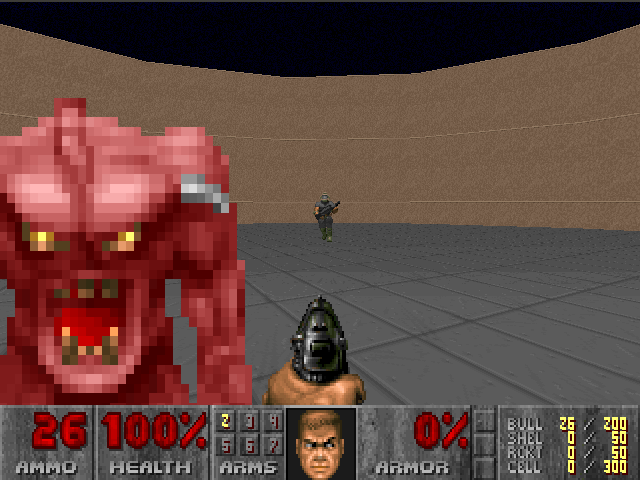
\includegraphics[scale=0.5]{defend_the_center.png}
		\caption{Doom gameplay frame from ''defend the center'' scenario}
	\end{figure}
\begin{itemize}
	\item motivation
	\item description
\end{itemize}

\newpage
\subsection{Defend the Line}
	\begin{figure}[h]
		\centering
		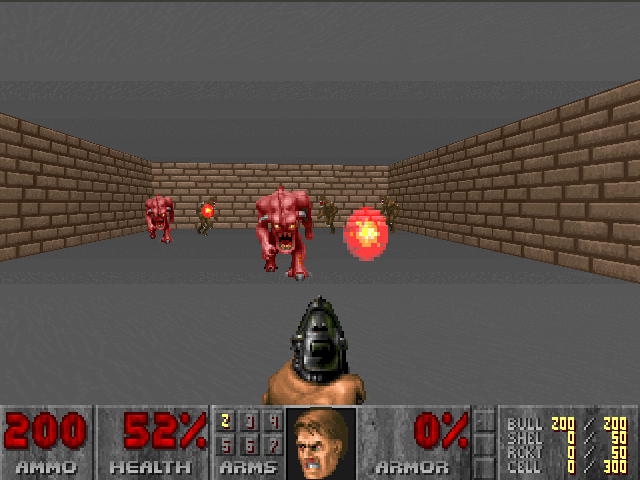
\includegraphics[scale=0.5]{defend_the_line.png}
		\caption{Doom gameplay frame from ''defend the line'' scenario}
	\end{figure}
\begin{itemize}
	\item motivation
	\item description
\end{itemize}

\newpage
\subsection{Deathmatch}
	GRAPHICS SOON
\begin{itemize}
	\item motivation
	\item description
\end{itemize}

\newpage
\subsection{Health Gathering}
	\begin{figure}[h]
		\centering
		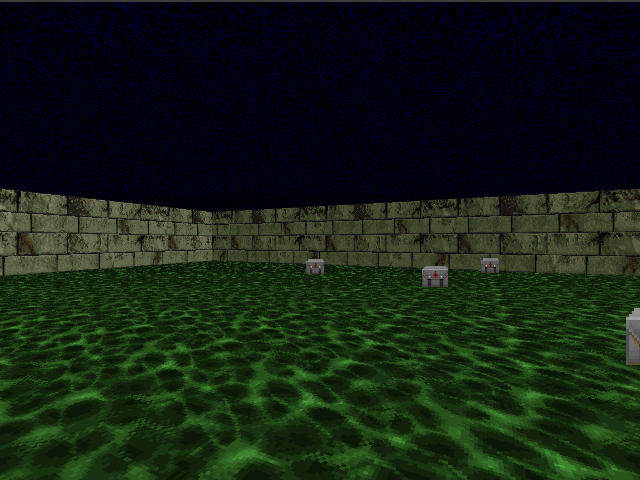
\includegraphics[scale=0.5]{health_gathering.png}
		\caption{Doom gameplay frame from ''health gathering'' scenario}
	\end{figure}
\begin{itemize}
	\item motivation
	\item description
\end{itemize}

\newpage
\subsection{My Way Home}
	\begin{figure}[h]
		\centering
		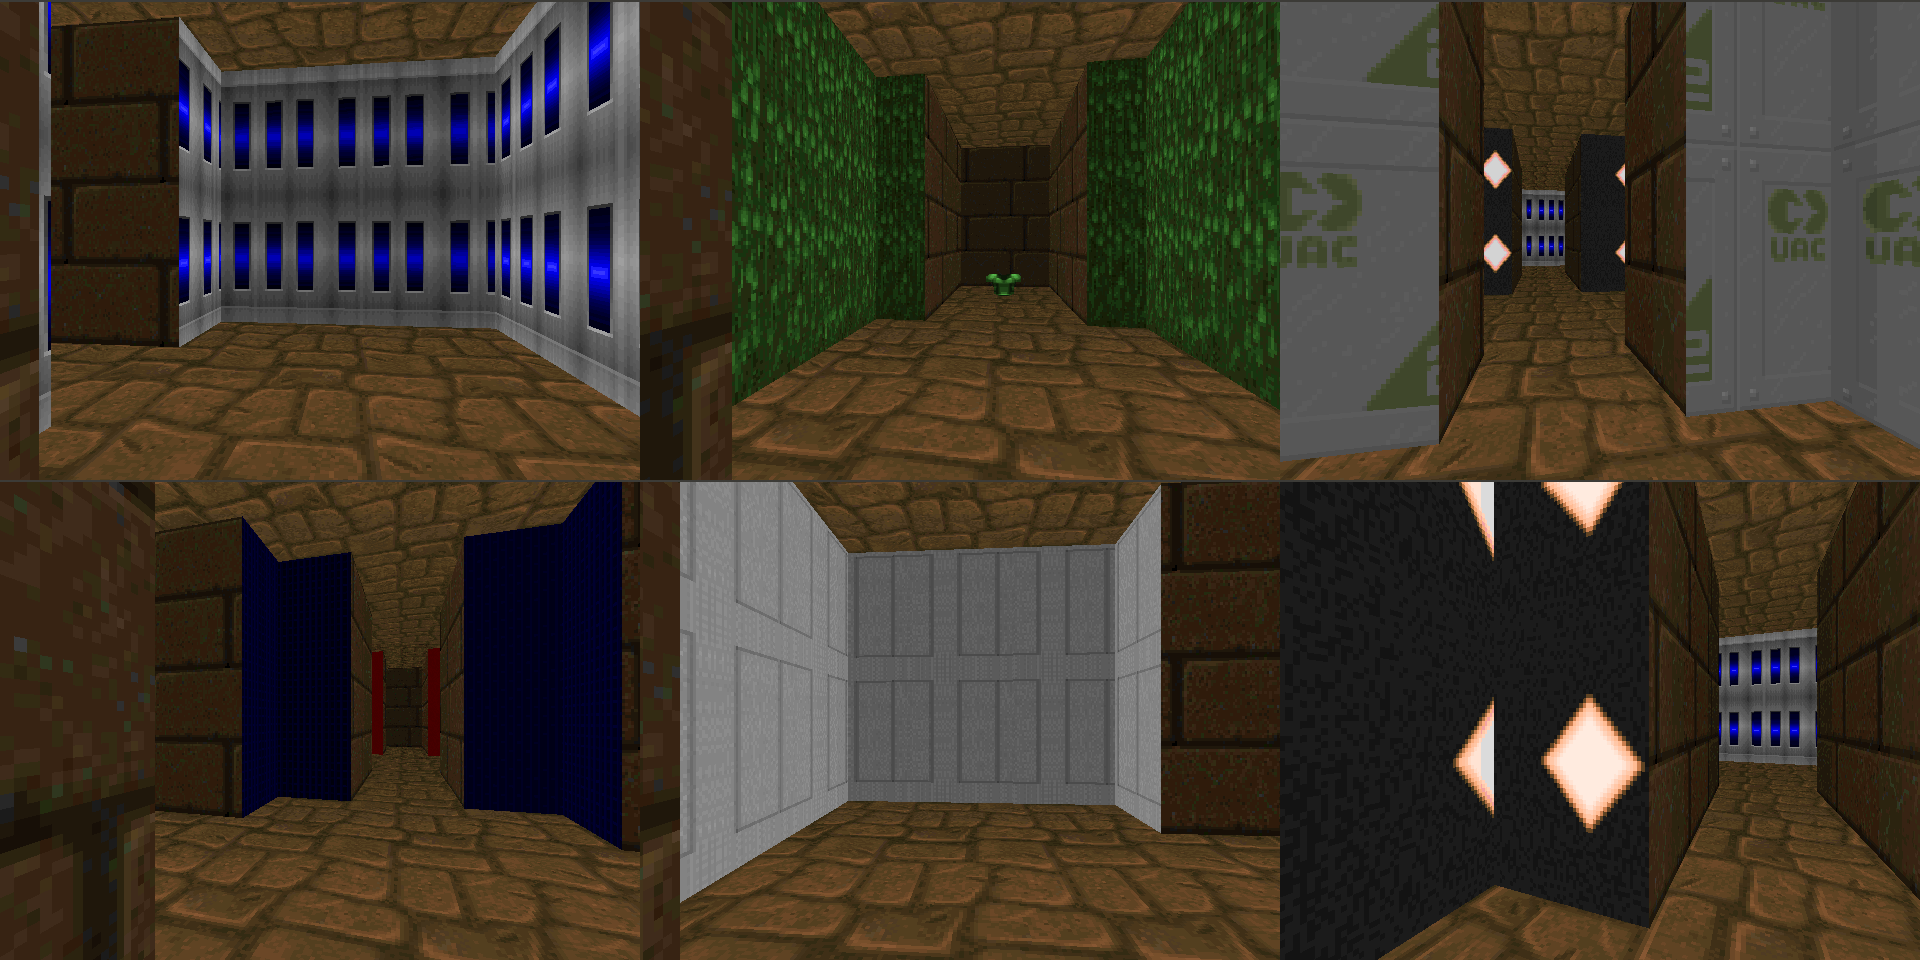
\includegraphics[scale=0.22]{my_way_home.png}
		\caption{6 random Doom gameplay frames from ''my way home'' scenario}
	\end{figure}
\begin{itemize}
	\item motivation
	\item description
\end{itemize}

\newpage
\subsection{Predict Position}
	\begin{figure}[h]
		\centering
		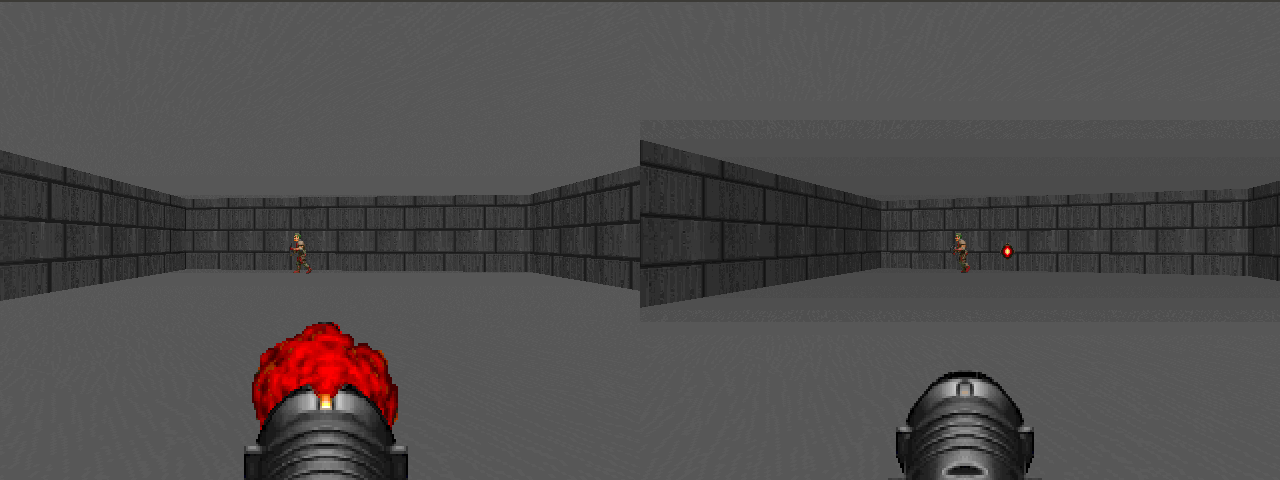
\includegraphics[scale=0.32]{predict_position.png}
		\caption{2 random Doom gameplay frames from ''predict position'' scenario}
	\end{figure}
\begin{itemize}
	\item motivation
	\item description
\end{itemize}

\newpage
\subsection{Take Cover}
	\begin{figure}[h]
		\centering
		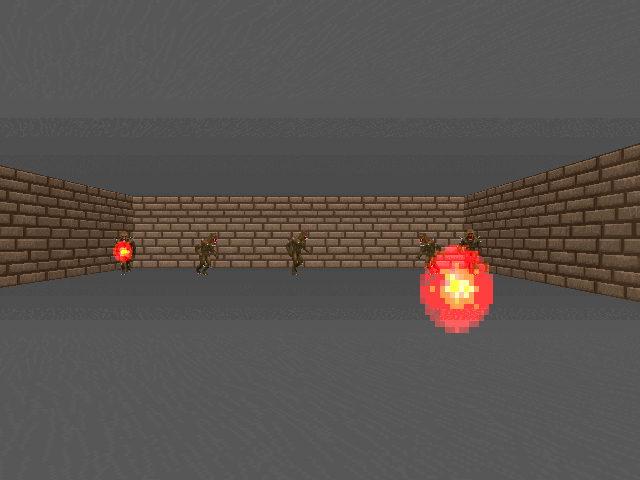
\includegraphics[scale=0.5]{take_cover.png}
		\caption{Doom gameplay frame from ''take cover'' scenario}
	\end{figure}
\begin{itemize}
	\item motivation
	\item description
\end{itemize}

